%!TEX root = ../slides2.tex
\section{Датасеты}
\begin{frame}
    \frametitle{Датасеты}
    \begin{itemize}
        \item A2D-Sentences: A Dataset and Benchmark for Action Recognition and Segmentation with Multiple Classes of Actors
        \begin{figure}
            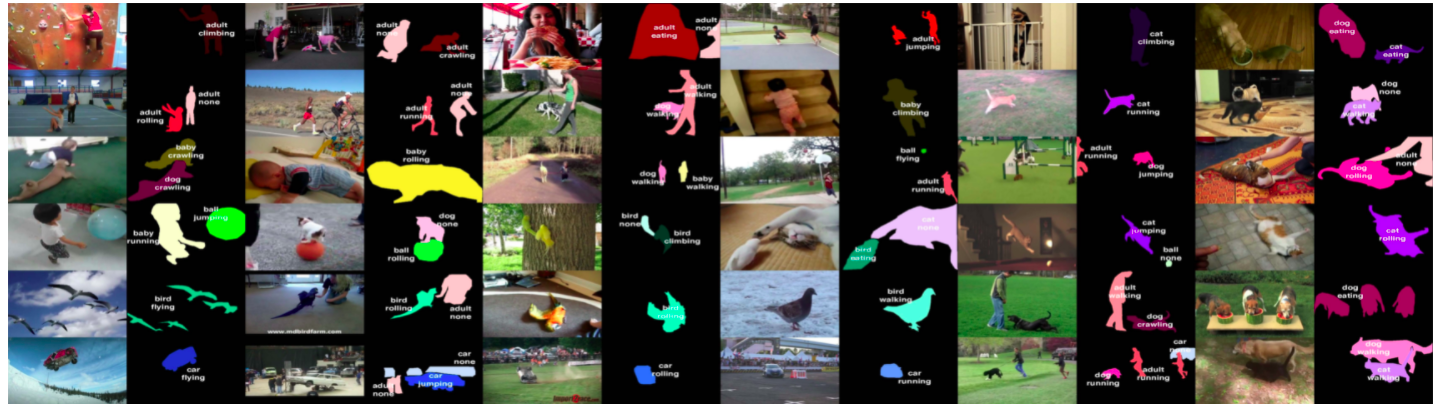
\includegraphics[scale=0.25]{a2d.png}
        \end{figure}
        \item JHMDB-Sentences: A fully annotated data set for human actions and human poses.
        \item Refer-YouTube-VOS
    \end{itemize}
\end{frame}

\section{Loss}
\begin{frame}
    \frametitle{Loss}
    \begin{itemize}
        \item \(\overline{y}=\{\overline{y_i}\}_{i=1}^{N}\)- множество предсказаний
        \item для каждого \(i\)
        предсказание имеет вид: \(\overline{y_i}=\{\overline{p}^t_i,\overline{b}^t_i, \overline{s}^t_i\}_{t=1}^T\)
        \item правильный ответ имеет вид: \(y=\{c^t,b^t,s^t\}_{t=1}^T\) 
        \begin{itemize}
            \item \(\overline{y}_{pos} = \underset{\overline{y_i}\in\overline{y}}{argmin} L_{match}(y, \overline{y_i})\)
            \item \(L_{match}(y, \overline{y_i})=k_{cls}L_{cls}(y, \overline{y_i})+
            k_{box}L_{box}(y, \overline{y_i})+ k_{mask}L_{mask}(y, \overline{y_i})\)
        \end{itemize}
    \end{itemize}
\end{frame}

\section{Метрики}
\subsection{IoU}
\begin{frame}
    \frametitle{Метрики}
    \begin{itemize}
        \item IoU:
         \begin{figure}
            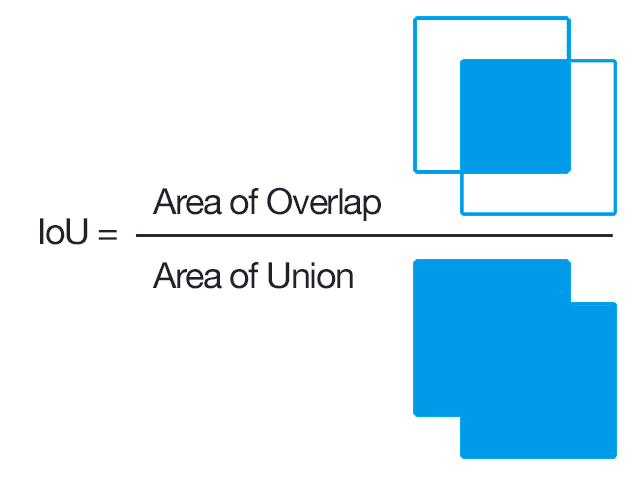
\includegraphics[scale=0.2]{iou.png}
        \end{figure}
        
    \end{itemize}
\end{frame}
\subsection{mAP}
\begin{frame}
    \frametitle{Метрики}
    \begin{itemize}
        \item \(mAP\):
        \begin{itemize}
            \item \(p=\frac{TP}{TP+FP}, \quad r=\frac{TP}{TP+FN}\)
            \item \(AP=\int_{0}^{1}p(r)dr\)
            \item \(mAP=\frac{1}{n}\sum_{i=1}^{n}AP_{i}, n -\)количество классов, \(AP_{i} - AP\) для \(i\)-го класса
        \end{itemize}

        \begin{figure}
            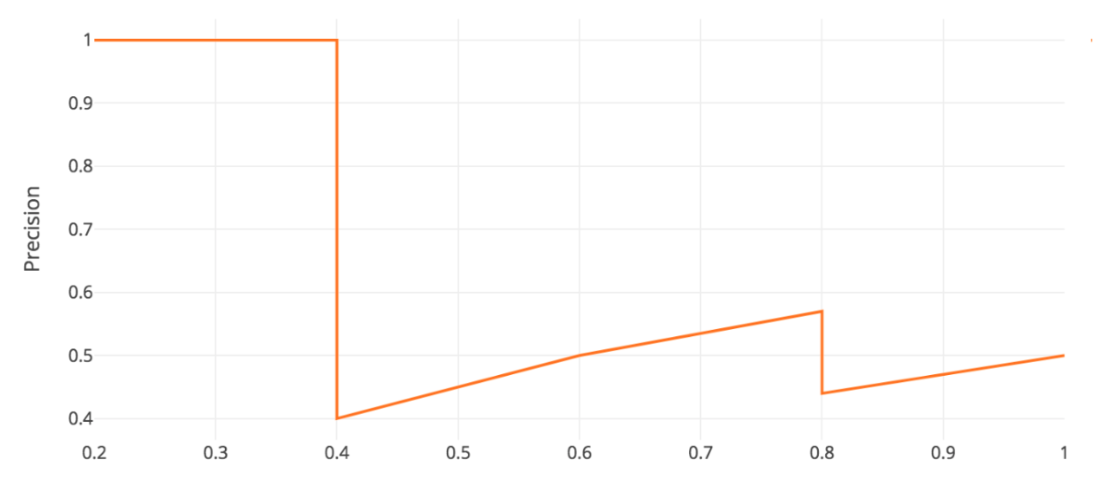
\includegraphics[scale=0.2]{prcurve.png}
        \end{figure}
    \end{itemize}
\end{frame}

\section{План работ}
\begin{frame}
    \frametitle{План работ}
    \begin{itemize}      
        \item Сделать обзор существующих методов сегментации объектов на видео по текстовому описанию - \textbf{сделано}.
        \item Запустить существующие решения - \textbf{сделано}.
        \item Рассмотреть идеи по улучшению или обобщению сегментации (например, bilingual - сегментация)
        \item Провести эксперименты
      
    \end{itemize}
\end{frame}


\begin{frame}
    \begin{center}
        \text{СПАСИБО ЗА ВНИМАНИЕ!}
    \end{center}
\end{frame}